\chapter{Manual de Instalación.}\label{sec:ManualDeInstalacion}

\paragraph{}En este capítulo se va a explicar cómo instalar el entorno de desarrollo
para cada uno de los principales sistemas operativos. Los pasos descritos se podrán
seguir con independencia del estado previo del sistema. No se asume ningún estado previo.

\section{Consideraciones previas}

\begin{itemize}
    \item El tecnologías y herramientas del entorno de desarrollo tienen como base
    sistemas operativos GNU/Linux, concretamente la versión 20.04 de la distribución
    de Ubuntu. Por lo que, a pesar de poder ser utilizados en cualquier sistema,
    serán en éstos donde será más fácil y óptimo su uso.

    \item Al igual que sucede en otros capítulos de este documento, se van a diferenciar
    las dos partes lógicas que componen el proyecto software: el entorno Flutter y el
    entorno Yocto.

    \item La inicaciones de este capítulo parten de sistemas con instalaciones por defecto
    y sin modificar, actualizados a la última versión disponible. Es posible que algún
    paso pueda variar, se pueda prescindir de algún paso, o que se requiera algún paso
    adicional, en función del tipo de instalación o versión.
\end{itemize}

\section{Instalación del entorno Flutter}\label{sec:entflutter}

\paragraph{}En el entorno Flutter vamos a ser capaces de desarrollar la aplicación,
pasar sus test y compilarla para diferentes plataformas.

\subsection{Instalación en sistemas operativos GNU/Linux}

\paragraph{}Para la instalación de este entorno en un sistema operativo basado en
la versión de Ubuntu 20.04 ó en la 22.04 se podrá optar por tres estrategias: correr
el entorno de forma nativa, utilizar el método basado en docker o utilizar la característica
de desarrollo en container de Visual Studio Code, que sería una solución intermedia.

\paragraph{}La instalación basada en desarrollo en container de Vscode, es posiblemente
el método más sencillo y rápido, tiene la ventaja que apenas modifica el sistema operativo
host y que cualquier cambio futuro en el entorno se actualizará con sólo actualizar el
propio repositorio. La instalación basada en docker, aunque conceptualmente es similar,
está pensado para usarse en infraestructura y procesos automatizados. Por último, la opción
nativa está recomendada para desarrolladores más avanzados que tengas permiso de administrador
y quieran tener el control sobre las herramientas base.

\subsection{Desarrollo en container de vscode.}

\paragraph{}\textbf{Nota:} Este método podría requerir permisos de \emph{sudo} o super
usuario en caso de que docker o Visual Studio Code no estén previamente instalados.

\begin{enumerate}
    \item Instalar \textbf{\gls{git}} (\emph{sólo si es necesario}).
    \begin{lstlisting}[style=consola, numbers=left]
        $ sudo apt install -y git
    \end{lstlisting}

    \item Clonar el repositorio desde github y entrar en el directorio.
    \begin{lstlisting}[style=consola, numbers=left]
        $ git clone https://github.com/Gmatarrubia/rpi_weather.git
        $ cd rpi_weather
    \end{lstlisting}

    \item Instalar Docker.
    \begin{lstlisting}[style=consola, numbers=left]
        $ source checkFunctions.sh
        $ check_docker
    \end{lstlisting}
    \textbf{Nota:} Después de este paso podría ser necesario reiniciar, la salida del
    script nos indicará si ésto fuera necesario. En caso de tener que reiniciar,
    podríamos continuar la instalación abriendo de nuevo una terminal, yendo al directorio
    del repositorio y reanudar la guía en el siguente paso.

    \item Instalar Visual Studio Code.
    \begin{lstlisting}[style=consola, numbers=left]
        $ source checkFunctions.sh
        $ check_vscode
    \end{lstlisting}

    \item Abrir el repositorio con \gls{vscode}
    \begin{lstlisting}[style=consola, numbers=left]
        $ code .
    \end{lstlisting}

    \item Reabrir la carpeta en el container como nos sugerirá.
    \begin{figure}[H]
        \centering
        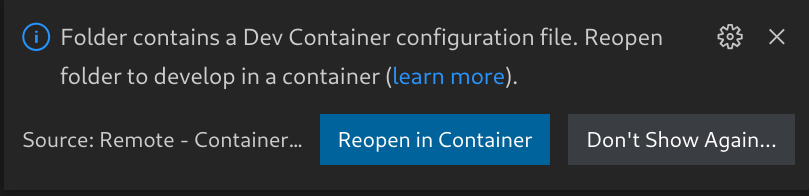
\includegraphics[width=0.55\textwidth]{imgs/dev-container}
        \caption[Mensaje emergente en vscode]{Mensaje emergente en vscode.}
        \label{imgs:vscode-devcontainer}
    \end{figure}

    \item Fin de la instalación. En caso de que no \gls{vscode} no detecte el \gls{SDK}
    reiniciar \gls{vscode} y volver a abrirlo y volver a seleccionar en ``abrir en container''.
\end{enumerate}

\subsection{Entorno de desarrollo dockerizado.}

\paragraph{}\textbf{Nota:} Este método podría requerir permisos de \emph{sudo} o super
usuario en caso de que docker no esté previamente instalado.

\begin{enumerate}
    \item Instalar \textbf{\gls{git}} (\emph{sólo si es necesario}).
    \begin{lstlisting}[style=consola, numbers=left]
        $ sudo apt install -y git
    \end{lstlisting}

    \item Clonar el repositorio desde github
    \begin{lstlisting}[style=consola, numbers=left]
        $ git clone https://github.com/Gmatarrubia/rpi_weather.git
        $ cd rpi_weather
    \end{lstlisting}

    \item (Opcional) En caso de necesitar instalar Visual Studio Code para el desarrollo,
    se puede utilizar la siguente opctión.
    \begin{lstlisting}[style=consola, numbers=left]
        $ source checkFunctions.sh
        $ check_vscode
    \end{lstlisting}

    \item Ejecutar el script inicialización de container. Este script construye la
    imagen en caso de que no haya sido creada previamente.
    \begin{lstlisting}[style=consola, numbers=left]
        $ ./init-docker-env.sh
    \end{lstlisting}
    \textbf{Nota:} Después de este paso podría ser necesario reiniciar, la salida del
    script nos indicará si ésto fuera necesario. Si reiniciamos, sería necesario volver
    a repetir este último paso para que la instalación continue.

    \item Ejecutar el script de obtención de dependencias.
    \begin{lstlisting}[style=consola, numbers=left]
        (docker)$ ./getSources.sh
    \end{lstlisting}

    \item Fin de la instalación.
\end{enumerate}

\begin{figure}[H]
    \centering
    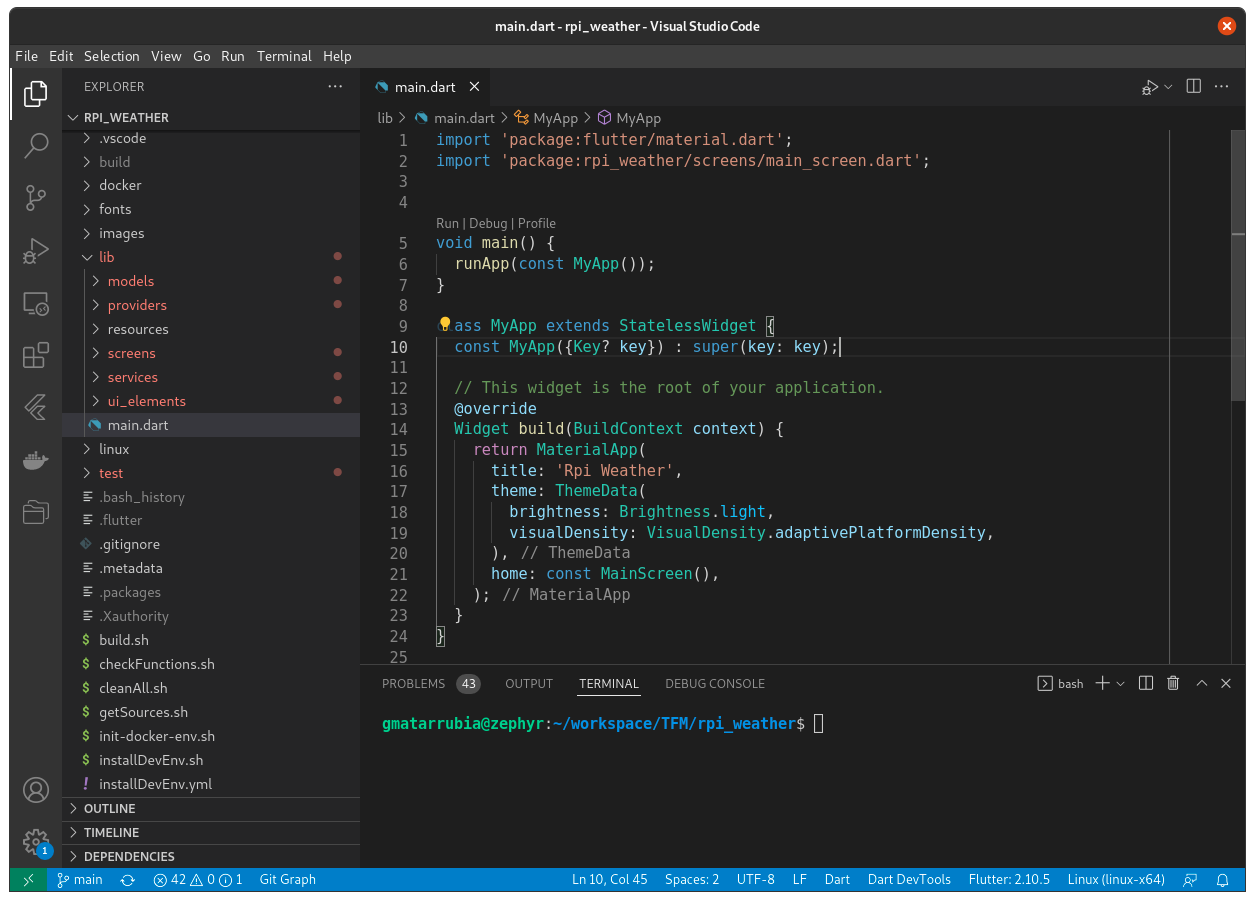
\includegraphics[width=0.95\textwidth]{imgs/vscode-ready}
	\caption[Visual Studio Code]{Visual Studio Code con el proyecto abierto.}
	\label{imgs:vscode-ready}
\end{figure}

\subsection{Instalación nativa.}

\paragraph{}\textbf{Nota:} Este método requiere permisos de \emph{sudo} o super usuario.

\begin{enumerate}
    \item Instalar \textbf{\gls{git}} (\emph{sólo si es necesario}).
    \begin{lstlisting}[style=consola, numbers=left]
        $ sudo apt install -y git
    \end{lstlisting}

    \item Clonar el repositorio desde github
    \begin{lstlisting}[style=consola, numbers=left]
        $ git clone https://github.com/Gmatarrubia/rpi_weather.git
        $ cd rpi_weather
    \end{lstlisting}

    \item Ejecutar el script de instalación de paquetes.
    \begin{lstlisting}[style=consola, numbers=left]
        $ sudo ./installDevEnv.sh
    \end{lstlisting}

    \item Ejecutar el script de obtención de dependencias.
    \begin{lstlisting}[style=consola, numbers=left]
        $ ./getSources.sh
    \end{lstlisting}

    \item (Opcional) En caso de necesitar instalar Visual Studio Code para el desarrollo,
    se puede utilizar la siguente opctión.
    \begin{lstlisting}[style=consola, numbers=left]
        $ source checkFunctions.sh
        $ check_vscode
    \end{lstlisting}

    \item Fin de la instalación.
\end{enumerate}

\subsection{Instalación en sistemas operativos Windows}\label{sec:install_win_flutter}

\paragraph{}Tanto Visual Studio Code, como el \gls{SDK} de Flutter tienen versiones
nativas para Windows. Aunque en principio, Flutter podría trabajar indistintamente en
versiones Windows y Linux de escritorio, para evitar posibles discrepancias en la
compatibilidad de dependencias se va a trabajar dentro de un entorno Linux llamado
\gls{WSL2}. Esta característica de Windows incluida en la versión 10 y 11 en ambos
casos en la ediciones pro, permite el uso de un sistema operativo basado en el kernel
de Linux dentro del propio sistema Windows sin virtualización del hardware.

\paragraph{}\textbf{Nota:} Se requieren permisos de administrador.

\paragraph{}Por tanto los pasos para obtener nuestro entorno de desarrollo listo para
trabajar son:

\begin{enumerate}
    \item Instalar y configurar \gls{WSL2}. Para ello, abrir una consola, ya sea cmd
    o powershell, con permisos de administrador e introducir el siguiente comando:
    \begin{lstlisting}[style=cmd, numbers=left]
        wsl.exe --install
    \end{lstlisting}

    \item Reiniciar el sistema.

    \item Arrancar \gls{WSL2} desde el Menú de Inicio. Y realizar la configuración
    inicial que se nos indique, normalmente esto consiste en crear un usuario y
    contraseña.

    \item Una vez en la terminal de \gls{WSL2}, comprobamos que todo haya ido bien realizando
    la actualización de los paquetes de sistema con:
    \begin{lstlisting}[style=consola, numbers=left]
        $ sudo apt update
        $ sudo apt upgrade
    \end{lstlisting}

    \item Siguiendo en la terminal de \gls{WSL2}, instalamos la herramienta git y clonamos
    el repositorio.
    \begin{lstlisting}[style=consola, numbers=left]
        $ sudo apt install -y git
        $ git clone https://github.com/Gmatarrubia/rpi_weather.git
    \end{lstlisting}

    \item Instalar Visual Studio Code siguiendo la instalación recomendada en su página
    oficial: \href{https://code.visualstudio.com/download}{https://code.visualstudio.com/download}

    \item Instalar una herramienta de escritorio remoto VNC que soporte tunneling SSH.
    Recomendablemente Gsshvnc, la cual se puede descargar aquí:
    \href{https://github.com/zrax/gsshvnc/releases}{Github Gsshvnc Releases}

    \begin{figure}[H]
        \centering
        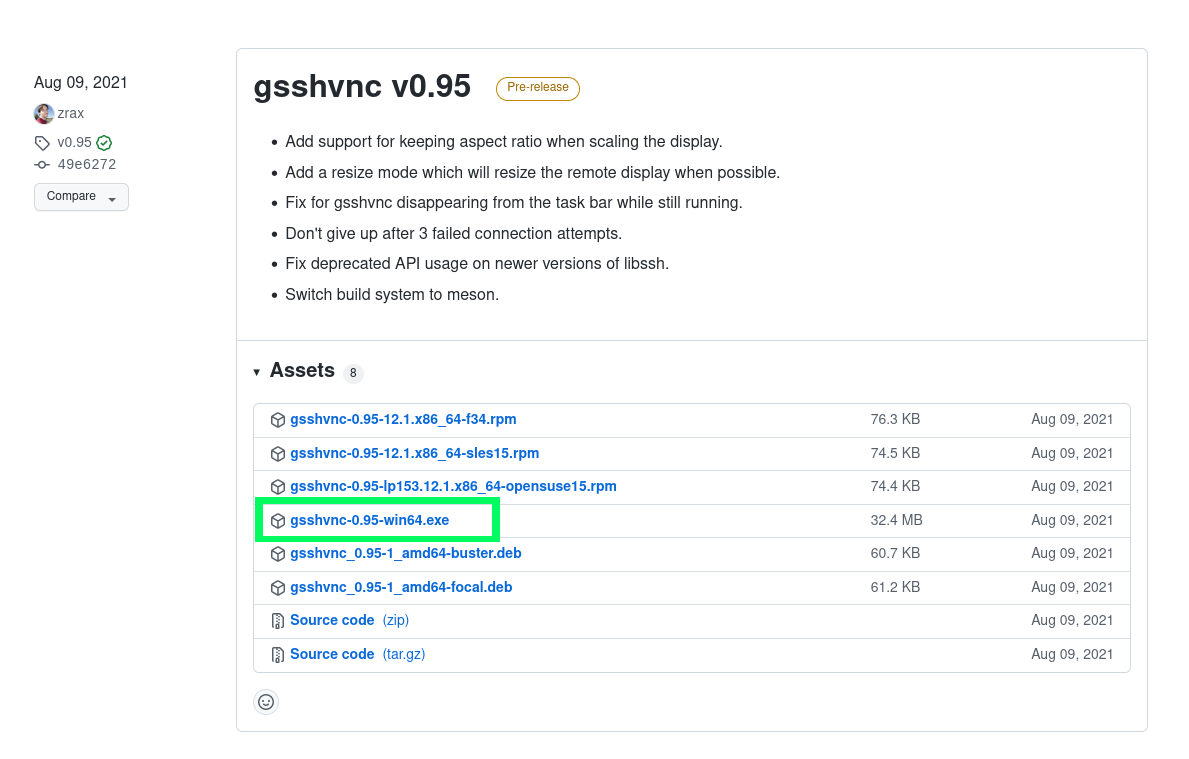
\includegraphics[width=0.95\textwidth]{imgs/gsshvnc-releases}
        \caption[gsshvnc releases]{gsshvnc página de descargas.}
        \label{imgs:gsshvnc-releases}
    \end{figure}

    \item Abrir Visual Studio Code e instalar las extensiones necesarias. Para ello
    una vez en VSCode, utilizar el atajo de teclado \emph{Ctrl+p} e introducir el siguiente
    comando. Debemos aceptar cualquier sugerencia que nos pregunte:
    \begin{lstlisting}[style=cmd]
        ext install ms-vscode-remote.vscode-remote-extensionpack
    \end{lstlisting}

    \item Abrir un entorno \gls{WSL2} en Visual Studio Code y abrir la carpeta del repositorio
    previamente descargado tal y como muestran las siguientes imágenes.

    \begin{figure}[H]
        \centering
        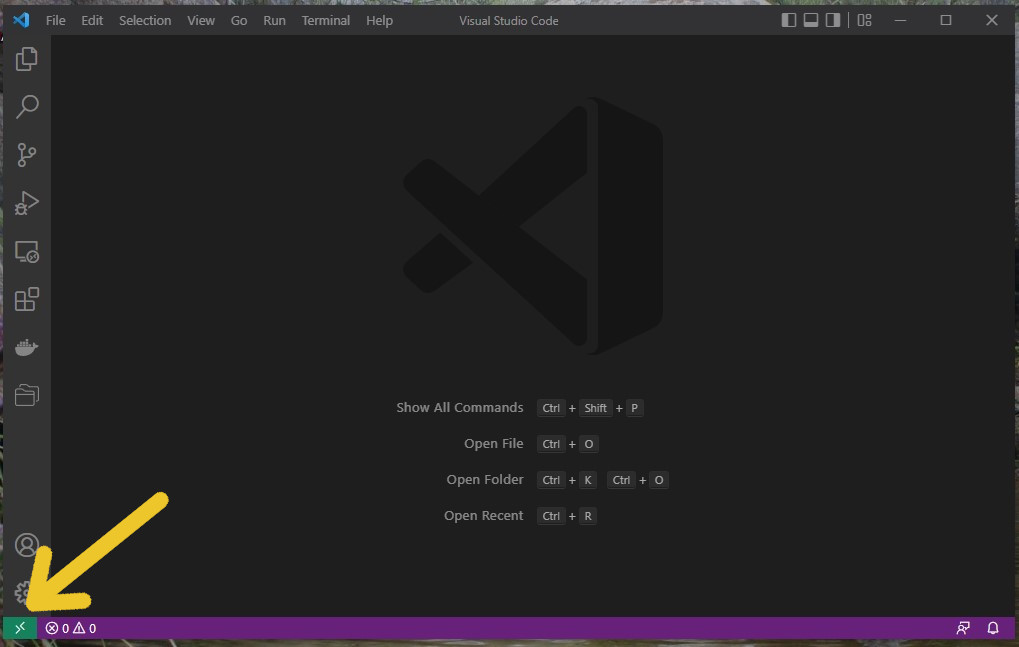
\includegraphics[width=0.95\textwidth]{imgs/vscode-wsl2}
        \caption[Botón para abrir Vscode en WSL2.]{Botón para abrir Vscode en WSL2.}
        \label{imgs:vscde-wsl2}
    \end{figure}

    \begin{figure}[H]
        \centering
        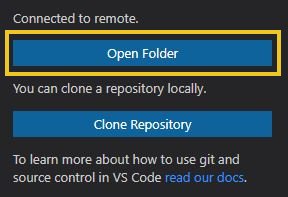
\includegraphics[width=0.55\textwidth]{imgs/vscode-wsl2-2}
        \caption[Abrir una carpeta.]{Abrir una carpeta.}
        \label{imgs:vscde-wsl2-2}
    \end{figure}

    \begin{figure}[H]
        \centering
        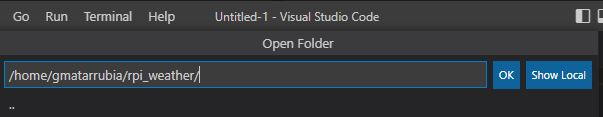
\includegraphics[width=0.95\textwidth]{imgs/vscode-wsl2-3}
        \caption[Selección de carpeta.]{Selección de carpeta.}
        \label{imgs:vscde-wsl2-3}
    \end{figure}

    \item Instalar la extension de Visual Studio Code de Flutter de la misma manera que
    en el paso anterior.
    \begin{lstlisting}[style=cmd]
        ext install Dart-Code.flutter
    \end{lstlisting}

    \item Ejecutar el script de instalación de paquetes.
    \begin{lstlisting}[style=consola, numbers=left]
        $ sudo ./installDevEnv.sh
    \end{lstlisting}

    \item Ejecutar el script de obtención de dependencias.
    \begin{lstlisting}[style=consola, numbers=left]
        $ ./getSources.sh
    \end{lstlisting}

    \item Reiniciar Visual Studio Code.

    \item Fin de la instalación.
\end{enumerate}

\subsection{Instalación en sistemas operativos MacOS.}

\paragraph{}\emph{De momento, la instalación en sistemas MacOS no es posible ya que
existen una serie de pequeñas incompatibilidades en el repositorio. Estas
incompatibilidades pueden arreglarse en el futuro o se pueden gestionar con una rama
de desarrollo en Mac a parte. De momento, lo más recomendable es crear una máquina
virtual Ubuntu 22.04 y utilizar la instalación nativa.}

\newpage
%%%%%%%%%%%%%%%%%%%%%%%%%%%%%%%%%%%%%%%%%%%%%%%%%%%%%%%%%%%%%%%%%%%%%%%%%%%%%%%

\section{Instalación del entorno Yocto}

\subsection{Instalación en sistemas operativos GNU/Linux}

\paragraph{}Al igual que sucedía con el entorno de Flutter \ref{sec:entflutter}, existe
la posibilidad de correr el entorno de manera nativa, de manera \emph{dockerizada} o
mediante el desarrollo en container de \gls{vscode}.
Ambos entornos se han diseñado para tener una instalación y usos parecidos y así que
se mantenga una coherencia común y una experiencia de usuario parecida, reduciendo así
la curva de aprendizaje y las barreras de entrada.

\subsection{Desarrollo en container de vscode.}

\paragraph{}\textbf{Nota:} Este método podría requerir permisos de \emph{sudo} o super
usuario en caso de que docker o Visual Studio Code no estén previamente instalados.

\begin{enumerate}
    \item Instalar \textbf{\gls{git}} (\emph{sólo si es necesario}).
    \begin{lstlisting}[style=consola, numbers=left]
        $ sudo apt install -y git
    \end{lstlisting}

    \item Clonar el repositorio desde github y entrar en el directorio.
    \begin{lstlisting}[style=consola, numbers=left]
        $ git clone https://github.com/Gmatarrubia/dev_env_rpi_flutter_yocto.git
        $ cd dev_env_rpi_flutter_yocto
    \end{lstlisting}

    \item Instalar Docker.
    \begin{lstlisting}[style=consola, numbers=left]
        $ source checkFunctions.sh
        $ check_docker
    \end{lstlisting}
    \textbf{Nota:} Después de este paso podría ser necesario reiniciar, la salida del
    script nos indicará si ésto fuera necesario. En caso de tener que reiniciar,
    podríamos continuar la instalación abriendo de nuevo una terminal, yendo al directorio
    del repositorio y reanudar la guía en el siguente paso.

    \item Instalar Visual Studio Code.
    \begin{lstlisting}[style=consola, numbers=left]
        $ source checkFunctions.sh
        $ check_vscode
    \end{lstlisting}

    \item Abrir el repositorio con \gls{vscode}
    \begin{lstlisting}[style=consola, numbers=left]
        $ code .
    \end{lstlisting}

    \item Reabrir la carpeta en el container como nos sugerirá.
    \begin{figure}[H]
        \centering
        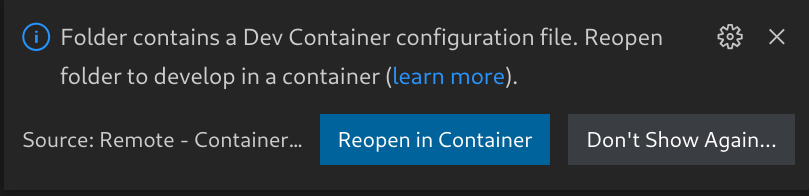
\includegraphics[width=0.55\textwidth]{imgs/dev-container}
        \caption[Mensaje emergente en vscode]{Mensaje emergente en vscode.}
        \label{imgs:vscode-devcontainer2}
    \end{figure}

    \item Fin de la instalación.
\end{enumerate}

\subsection{Instalación basada en docker.}

\paragraph{}\textbf{Nota:} Este método requiere permisos de \emph{sudo} o super usuario
usuario en caso de que docker no esté previamente instalado.

\begin{enumerate}
    \item Instalar \textbf{\gls{git}} (\emph{sólo si es necesario}).
    \begin{lstlisting}[style=consola, numbers=left]
        $ sudo apt install -y git
    \end{lstlisting}

    \item Clonar el repositorio desde github
    \begin{lstlisting}[style=consola, numbers=left]
        $ git clone https://github.com/Gmatarrubia/dev_env_rpi_flutter_yocto.git
        $ cd dev_env_rpi_flutter_yocto
    \end{lstlisting}

    \item (Opcional) En caso de necesitar instalar Visual Studio Code para el desarrollo,
    se puede utilizar la siguente opctión.
    \begin{lstlisting}[style=consola, numbers=left]
        $ source checkFunctions.sh
        $ check_vscode
    \end{lstlisting}

    \item Ejecutar el script inicialización de container. Este script construye la
    imagen en caso de que no haya sido creada previamente.
    \begin{lstlisting}[style=consola, numbers=left]
        $ ./init-docker-env.sh
    \end{lstlisting}
    \textbf{Nota:} Después de este paso podría ser necesario reiniciar, la salida del
    script nos indicará si ésto fuera necesario. Si reiniciamos, sería necesario volver
    a repetir este último paso para que la instalación continue.

    \item Fin de la instalación.
\end{enumerate}

\begin{figure}[H]
    \centering
    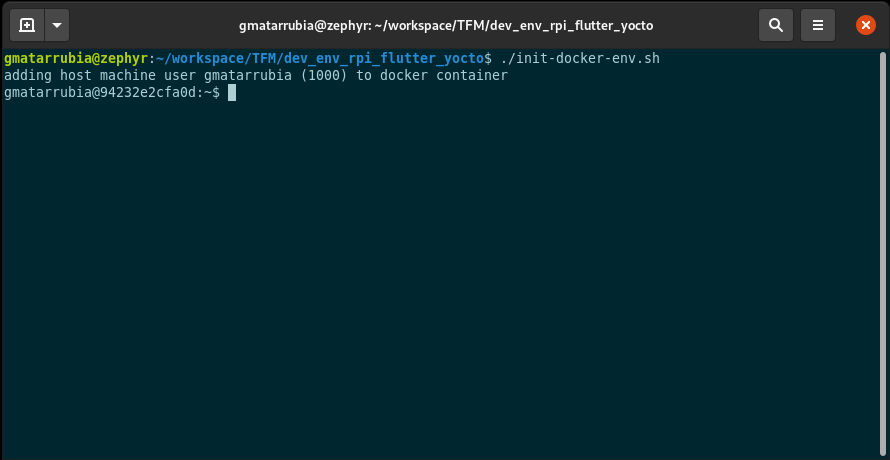
\includegraphics[width=0.95\textwidth]{imgs/yocto-docker-ready}
    \caption[yocto docker ready]{Entorno de desarrollo Yocto listo.}
    \label{imgs:yocto-docker-ready}
\end{figure}

\subsection{Instalación nativa.}

\paragraph{}\textbf{Nota:} Este método requiere permisos de \emph{sudo} o super usuario.

\begin{enumerate}
    \item Instalar \textbf{\gls{git}} (\emph{sólo si es necesario}).
    \begin{lstlisting}[style=consola, numbers=left]
        $ sudo apt install -y git
    \end{lstlisting}

    \item Clonar el repositorio desde github
    \begin{lstlisting}[style=consola, numbers=left]
        $ git clone https://github.com/Gmatarrubia/dev_env_rpi_flutter_yocto.git
    \end{lstlisting}

    \item Ejecutar el script de instalación de paquetes.
    \begin{lstlisting}[style=consola, numbers=left]
        $ cd dev_env_rpi_flutter_yocto
        $ sudo ./installDevEnv.sh
    \end{lstlisting}

    \item (Opcional) En caso de necesitar instalar Visual Studio Code para el desarrollo,
    se puede utilizar la siguente opctión.
    \begin{lstlisting}[style=consola, numbers=left]
        $ source checkFunctions.sh
        $ check_vscode
    \end{lstlisting}

    \item Fin de la instalación.
\end{enumerate}

\subsection{Instalación en sistemas operativos Windows.}

\paragraph{}\textbf{Nota:} Este método es una prueba de concepto y el rendimiento puede
verse visiblemente afectado. Como opción alternativa se aconseja crear una máquina
virtual Ubuntu 22.04 y seguir los consejos de la instalación en Linux de manera nativa.

\paragraph{}\textbf{Nota 2:} Se requieren permisos de administrador.

\paragraph{}Los pasos para obtener nuestro entorno de desarrollo listo para trabajar son:

\begin{enumerate}
    \item Instalar y configurar \gls{WSL2}. Para ello, abrir una consola, ya sea cmd
    o powershell, con permisos de administrador e introducir el siguiente comando:
    \begin{lstlisting}[style=cmd, numbers=left]
        wsl.exe --install
    \end{lstlisting}

    \item Reiniciar el sistema.

    \item Arrancar \gls{WSL2} desde el Menú de Inicio. Y realizar la configuración
    inicial que se nos indique, normalmente esto consiste en crear un usuario y
    contraseña.

    \item Una vez en la terminal de \gls{WSL2}, comprobamos que todo haya ido bien realizando
    la actulización de los paquetes de sistema con:
    \begin{lstlisting}[style=consola, numbers=left]
        $ sudo apt update
        $ sudo apt upgrade
    \end{lstlisting}

    \item Siguiendo en la terminal de \gls{WSL2}, instalamos la herramienta git y clonamos
    el repositorio.
    \begin{lstlisting}[style=consola, numbers=left]
        $ sudo apt install -y git
        $ git clone https://github.com/Gmatarrubia/dev_env_rpi_flutter_yocto.git
    \end{lstlisting}

    \item Instalar Visual Studio Code siguiendo la instalación recomendada en su página
    oficial: \href{https://code.visualstudio.com/download}{https://code.visualstudio.com/download}

    \item Abrir Visual Studio Code e instalar las extensiones necesarias. Para ello
    una vez en VSCode, utilizar el atajo de teclado \emph{Ctrl+p} e introducir el siguiente
    comando. Debemos aceptar cualquier sugerencia que nos pregunte:
    \begin{lstlisting}[style=cmd]
        ext install ms-vscode-remote.vscode-remote-extensionpack
    \end{lstlisting}

    \item Abrir un entorno \gls{WSL2} en Visual Studio Code y abrir la carpeta del repositorio
    previamente descargado tal y como muestran las siguientes imágenes.

    \begin{figure}[H]
        \centering
        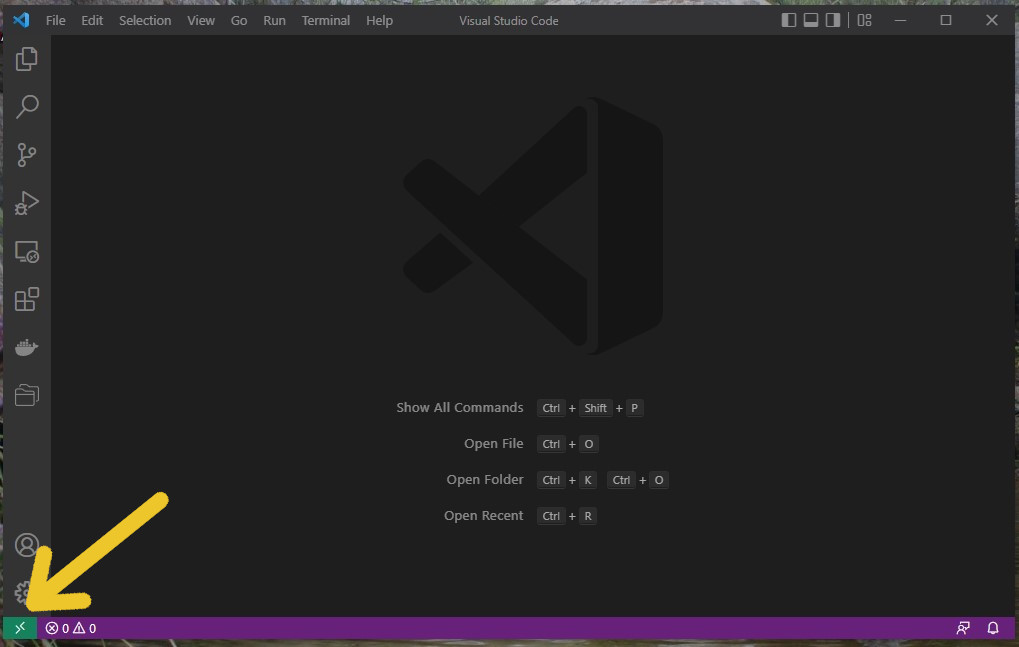
\includegraphics[width=0.95\textwidth]{imgs/vscode-wsl2}
        \caption[Botón para abrir Vscode en WSL2.]{Botón para abrir Vscode en WSL2.}
        \label{imgs:vscode-wsl2}
    \end{figure}

    \begin{figure}[H]
        \centering
        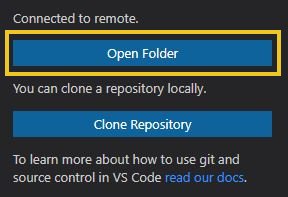
\includegraphics[width=0.55\textwidth]{imgs/vscode-wsl2-2}
        \caption[Abrir una carpeta.]{Abrir una carpeta.}
        \label{imgs:vscode-wsl2-2}
    \end{figure}

    \begin{figure}[H]
        \centering
        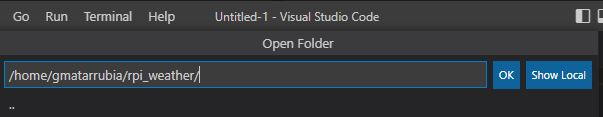
\includegraphics[width=0.95\textwidth]{imgs/vscode-wsl2-3}
        \caption[Selección de carpeta.]{Selección de carpeta.}
        \label{imgs:vscode-wsl2-3}
    \end{figure}

    \item Ejecutar el script de instalación de paquetes.
    \begin{lstlisting}[style=consola, numbers=left]
        $ sudo ./installDevEnv.sh
    \end{lstlisting}

    \item Fin de la instalación.
\end{enumerate}

\subsection{Instalación en sistemas operativos MacOS.}

\paragraph{}\emph{De momento, la instalación en sistemas MacOS no es posible ya que
existen una serie de incompatibilidades en el repositorio. Estas incompatibilidades
pueden arreglarse en el futuro o se pueden gestionar con una rama de desarrollo en Mac
a parte. De momento, lo más recomendable es crear una máquina virtual Ubuntu 22.04 y
utilizar la instalación nativa.}

%las referencias a artículos se ponen con \cite,
%las referencias a glosario \gls,
%y las referencias a ecuaciones \eqref
%las referencias a imgenes, tablas o figuras o secciones
% se ponen con \ref (sólo número) o con \hyperref[sec:X]{text}
